\chapter{Komunikace s~modelem auta}
\label{sec:PlatformCommunication}\

V~této kapitole je popsán způsob zobrazení a~ukládání dat během jízdy.

Během jízdy je důležité posílat data asynchronně, aby nebyl blokován hlavní
algoritmus auta. Z~toho důvodu pro komunikaci s~platformou je použit \textbf{UDP}
(User Datagram Protocol) protokol, který se primárně používá pro časově citlivé
informace. Zrychluje komunikaci tím, že před přenosem dat není nutné formálně
navazovat spojení, což umožňuje velmi rychlý přenos dat \cite{UDP}.

Během komunikace se vývojová deska chová jako UDP server a~klient pro server je
aplikací sloužící k~zobrazení dat. Aplikace pro zobrazení dat byla pojmenována jako
CarQt. \textbf{CarQt} umí zobrazovat originální obraz, normalizovány obraz
a~prahovaný obraz. Informace o~Regionech, PWM~motorech, servo motorech a~senzorech
jsou zobrazeny v~číselném formátu. Ukládání číselných dat je implementováno ve
formátu \textbf{JSON} (JavaScript Object Notation) a~originálního obrazu ve formátu
\textbf{PNG}~(Portable Network Graphics) souboru. Ukládaní do formátu JSON je napsáno pomocí knihovny JsonCpp. CarQt je napsána pomocí knihoven
Qt, JsonCpp a~OpenCV. Aplikace je zobrazena na obrázku \ref{fig:CarQt}.

\begin{figure}[!h]
    \centering
    \vspace{-10pt}
    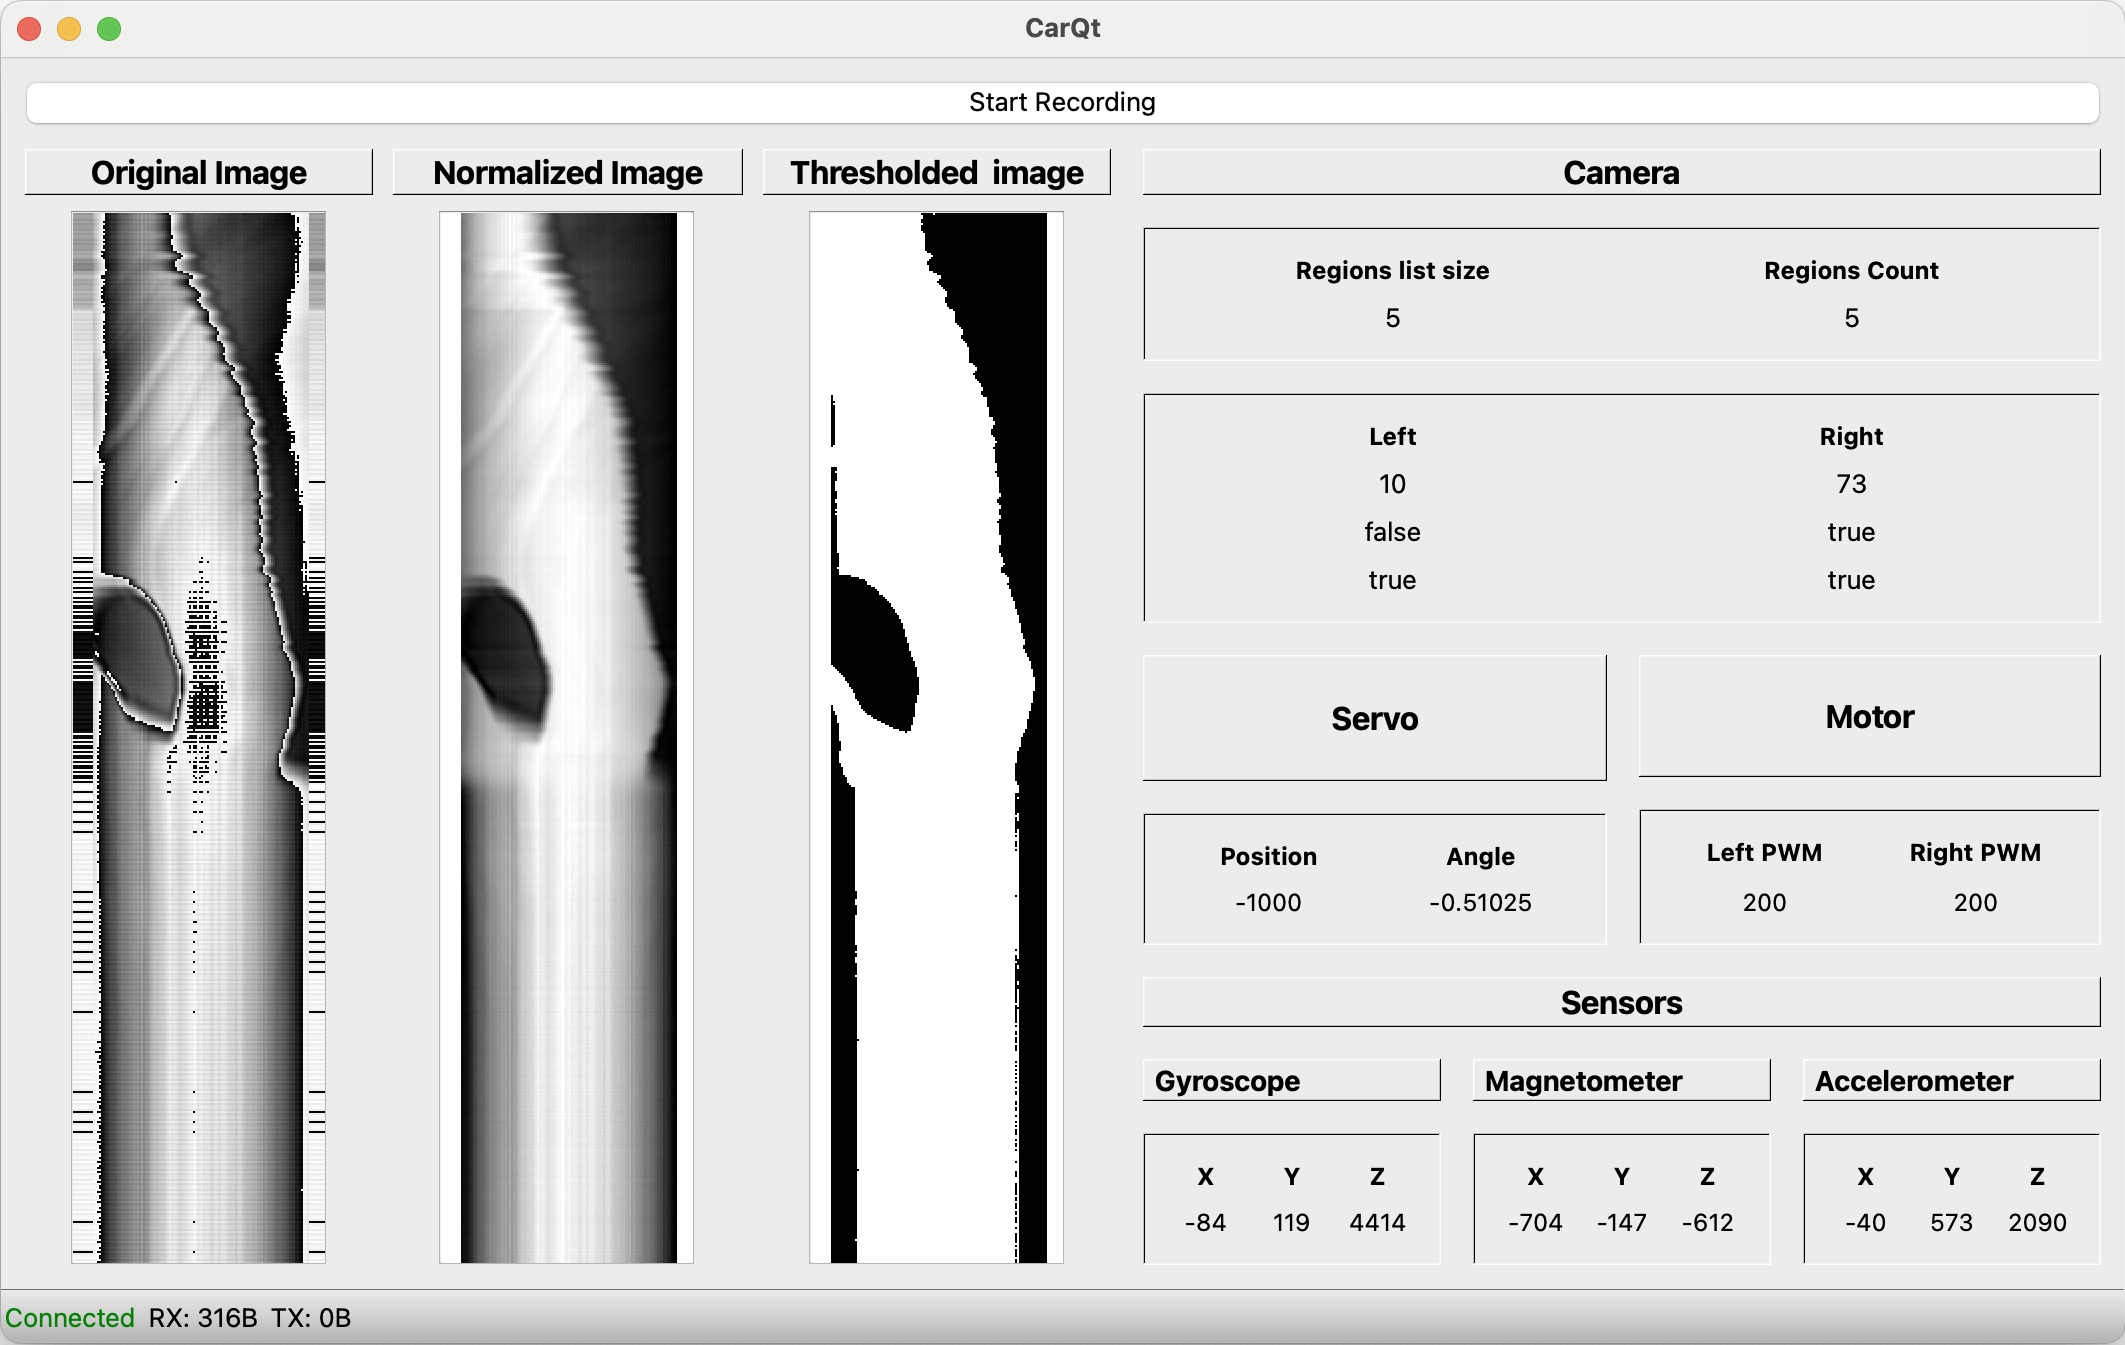
\includegraphics[width = .8\linewidth]{Figures/CarQt.png}
    \caption{CarQt aplikace.}
    \label{fig:CarQt}
    \vspace{-15pt}
\end{figure}

Pro přenos a~ukládání dat je použita struktura \textbf{Data}, která obsahuje:
\begin{itemize}
    \item originální data z~kamery,
    \item distance do levé i~pravé černé čáry,
    \item PWM hodnoty motorů,
    \item pozice a~úhel servomotoru,
    \item orientace senzorů,
    \item počet regionů.
\end{itemize}

Popis regionu je v~podkapitole \ref{sec:servocontrol}.
Implementovaná struktura Data je ve výpisu \ref{lst:data}.
\begin{lstlisting}[caption = Struktura Data, label = lst:data]
struct Data {
    uint16_t line[Image::LINE_LENGTH] = {0};
    uint32_t regionsCount = 0;
    uint32_t regionsListSize = 0;
    bool unchangedLeft = false;
    bool unchangedRight = false;
    bool hasLeft = false;
    bool hasRight = false;
    uint8_t leftDistance = 0;
    uint8_t rightDistance = 0;
    int32_t leftSpeed = 0;
    int32_t rightSpeed = 0;
    int32_t servoPosition = 0;
    float angle = .0f;
    Vec3<int16_t> accel = {0, 0, 0};
    Vec3<int16_t> mag = {0, 0, 0};
    Vec3<int16_t> gyro = {0, 0, 0};
    uint32_t timestamp = 0;
    uint8_t mode = Mode::None;
};
\end{lstlisting}

Praxe ukázala potřebnost nastavení adres pro přenos dat. Proto aplikace umožňuje nastavit adresy počítače i~MCU, port a~cestu pro ukládání dat. Nastavení se ukládají ve formátu JSON. Okno nastavení je zobrazeno na obrázku \ref{fig:CarQtSettings}.
\begin{figure}[!h]
\centering
    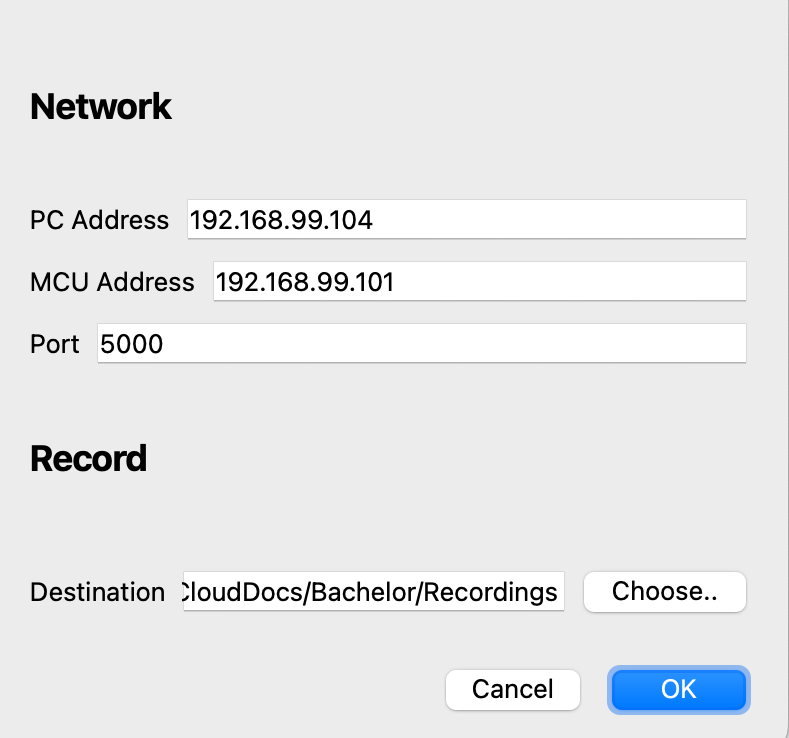
\includegraphics[width = .5\linewidth]{Figures/SettingsWindow.png}
\caption{Nastávení aplikace CarQt.}
\label{fig:CarQtSettings}
\end{figure}

\endinput